\documentclass[conference]{IEEEtran}
\IEEEoverridecommandlockouts

% ==========================================
% PACKAGES
% ==========================================
\usepackage{cite}
\usepackage{amsmath,amssymb,amsfonts}
\usepackage{algorithmic}
\usepackage{algorithm}
\usepackage{graphicx}
\usepackage{textcomp}
\usepackage{xcolor}
\usepackage{booktabs}
\usepackage{multirow}
\usepackage{float}
\usepackage{listings}
\usepackage{url}

% --- TIKZ & PLOTS SETUP ---
\usepackage{tikz}
\usepackage{pgfplots}
\pgfplotsset{compat=1.17}
\usetikzlibrary{shapes.geometric, arrows, positioning, fit, calc, backgrounds, er, automata}

% --- SAFE COMMAND DEFINITION ---
\providecommand{\RETURN}{\STATE \textbf{return} }

% --- COMPRESSION & SPACING FIXES ---
\setlength{\textfloatsep}{10pt plus 1.0pt minus 2.0pt}
\renewcommand{\baselinestretch}{1.0} 
\raggedbottom % Prevents LaTeX from aggressively stretching vertical spaces

% Force tight equation spacing globally to stop huge gaps
\makeatletter
\g@addto@macro\normalsize{%
  \setlength\abovedisplayskip{4pt plus 2pt minus 2pt}
  \setlength\belowdisplayskip{4pt plus 2pt minus 2pt}
  \setlength\abovedisplayshortskip{2pt plus 2pt minus 2pt}
  \setlength\belowdisplayshortskip{2pt plus 2pt minus 2pt}
}
\makeatother

% --- CODE LISTING STYLE ---
\lstset{
  basicstyle=\ttfamily\scriptsize,
  columns=fullflexible,
  breaklines=true,
  captionpos=b,
  frame=lines,
  numbers=left,
  numberstyle=\tiny\color{gray},
  keywordstyle=\color{blue},
  commentstyle=\color{green!50!black},
  stringstyle=\color{red},
  xleftmargin=1.5em,
  framexleftmargin=1em,
  aboveskip=0.3em,
  belowskip=0.3em
}

\def\BibTeX{{\rm B\kern-.05em{\sc i\kern-.025em b}\kern-.08em
    T\kern-.1667em\lower.7ex\hbox{E}\kern-.125emX}}

\begin{document}

% ==========================================
% TITLE
% ==========================================
\title{Real-Time Schedule Compliance via Spatiotemporal Predicate Evaluation and Relational Lookup}

% ==========================================
% AUTHOR & AFFILIATION
% ==========================================
\author{\IEEEauthorblockN{Dr. S. Suresh Kumar}
\IEEEauthorblockA{\textit{Department of Computer Science} \\
\textit{Swarnandhra College of Engineering \& Technology (Autonomous)}\\
Seetharampuram, Narsapur, Andhra Pradesh, India}
}

\maketitle

% ==========================================
% ABSTRACT
% ==========================================
\begin{abstract}
Modern campus environments increasingly deploy sensing infrastructure capable of identifying individuals and tracking spatial presence in real time. However, these sensing systems typically operate independently from institutional scheduling databases, preventing automated evaluation of whether detected presence aligns with scheduled academic obligations. This work presents a relational evaluation framework that reconciles spatial detection events with institutional schedules to enable continuous compliance evaluation.

We introduce the Continuous Predicate Evaluation Model (CPEM), which represents institutional rules as relational predicates evaluated over streaming event tuples. To reduce spurious violations caused by short-lived sensor noise, the evaluation logic incorporates a Persistent Constraint Violation Filter (PCVF) that smooths logical state transitions over time. Spatial exclusivity constraints further prevent inconsistent multi-zone detections from propagating into the evaluation layer.

To sustain synchronized burst traffic during class transitions, the evaluation logic integrates transaction-level connection pooling, list-based table partitioning, and composite temporal indexing within PostgreSQL. Experimental load testing demonstrates that continuous schedule reconciliation can be implemented using relational evaluation mechanisms while maintaining interactive latency under burst campus traffic conditions. The proposed analysis demonstrates that structured relational queries can process dynamic workloads at scale.
\end{abstract}

\begin{IEEEkeywords}
Schedule Compliance, Data Fusion, Spatiotemporal Analysis, Relational Databases, PostgreSQL, Signal Processing.
\end{IEEEkeywords}

% ==========================================
% I. INTRODUCTION
% ==========================================
\section{Introduction}

\subsection{The Semantic Gap in Campus Monitoring}
Large institutional campuses increasingly rely on sensing infrastructure to observe movement across classrooms, laboratories, and public spaces. While these systems can detect presence with high reliability, they typically lack direct integration with institutional scheduling data. As a result, sensing systems report location events without determining whether those events correspond to legitimate scheduled activity.

This separation between sensing infrastructure and administrative scheduling creates an operational gap. In early deployments, this disconnect was immediately apparent. The sensing layer reliably reported location, but the schedule database had no mechanism to react dynamically. The two systems operated in parallel rather than in coordination. This separation can therefore be interpreted as a semantic gap: perception without policy enforcement, and policy without live feedback. Effective relational evaluation models therefore become critical for maintaining consistent logical states. 

Attendance procedures further compound the issue. Faculty often record attendance at the start of a session, after which presence is typically assumed rather than continuously verified. Students may exit shortly after roll call while remaining marked “present” in static records. Without continuous reconciliation between schedule and location, mid-session deviations go undetected.

\subsection{Continuous Logic Evaluation}
Closing this operational gap requires rethinking how schedule compliance is evaluated. Traditional attendance systems typically rely on discrete, single-point verification events—an ID swipe or biometric check at entry. Such mechanisms confirm presence at one instant but provide no visibility into subsequent behavior.

The proposed logic treats presence as a stream rather than a snapshot. Compliance logic executes continuously over event tuples \cite{b14}, enabling detection of mid-session deviations and unauthorized zone occupancy. Instead of verifying “Was the student here at 9:00?”, the logic evaluates “Is the student where they are expected to be right now?” This shift from static verification to ongoing predicate evaluation broadly aligns with real-time stream processing principles \cite{b13}.

\subsection{Contributions}
Implementing continuous compliance evaluation required several adaptations within the relational pipeline. The primary focus of this work is the data evaluation logic necessary to make continuous compliance evaluation viable at institutional scale.

Specifically, this paper:
\begin{itemize}
    \item Formalizes campus adherence rules as continuously evaluated relational predicates (CPEM), enabling schedule comparison at event granularity.
    \item Introduces a temporally smoothed violation mechanism (PCVF) to suppress short-lived mismatches caused by transit or sensor instability.
    \item Establishes spatial exclusivity invariants to guard against inconsistent upstream detections.
    \item Optimizes relational read paths using connection pooling, table partitioning, and composite indexing to sustain burst concurrency.
\end{itemize}

Biometric extraction and identity resolution are treated as upstream dependencies; the present work isolates the relational fusion and evaluation layer.

% ==========================================
% II. RELATED WORK
% ==========================================
\section{Related Work}

\subsection{Limitations of Passive Evaluation}
Existing institutional monitoring systems often emphasize detection accuracy but provide limited mechanisms for real-time policy enforcement. Much institutional infrastructure is designed primarily for post-event analysis rather than live enforcement. Psychophysical studies suggest that sustained human monitoring degrades significantly over extended observation periods. Without automated filtering mechanisms, most relevant anomalies remain unnoticed \cite{b7}. Moreover, manually correlating observed identities with dynamic timetables is operationally impractical at scale.

The approach developed here emphasizes exception-based evaluation. Human attention is engaged only when a formally defined deviation occurs \cite{b17}, reducing monitoring burden while preserving responsiveness.

\subsection{Automated Attendance vs. Continuous Evaluation}
RFID badges and biometric entry systems verify presence at specific checkpoints \cite{b2, b3}. These systems log facility entry but do not track subsequent movement. Once marked present, a student’s status typically remains static until manually updated.

Continuous zone-based evaluation can extend this model. By integrating moving-object database principles \cite{b15, b16}, the logic dynamically evaluates adherence throughout the session rather than at a single timestamp.

\subsection{Smart Campus Data Fusion}
Recent Smart Campus initiatives emphasize dense IoT integration to improve operational visibility \cite{b1}. Multimodal fusion approaches have enhanced situational awareness across domains \cite{b6}. The present work applies similar fusion principles specifically to schedule adherence, securely integrating detection events \cite{b23} with centralized relational records.

Rather than optimizing perception, the emphasis in this work is on logical reconciliation.

% ==========================================
% III. OPERATIONAL MODEL
% ==========================================
\section{Operational Model}

\subsection{Context-Blindness in Edge Sensors}
Edge detection systems are typically optimized for perception tasks rather than policy interpretation \cite{b5}. They can identify an opaque identity token and associate it with a specific zone at a given timestamp, but they cannot determine whether that presence is legitimate relative to institutional rules.

Consider two identical physical observations at 14:30:
\begin{itemize}
    \item \textbf{Scenario A:} Student $X$ is detected at the Exit Gate. The schedule indicates campus dismissal. $\rightarrow$ \textit{Evaluation: Compliant.}
    \item \textbf{Scenario B:} Student $X$ is detected at the Exit Gate. The schedule indicates mandatory laboratory. $\rightarrow$ \textit{Evaluation: Non-compliant.}
\end{itemize}

From the sensor’s perspective, both observations are equivalent. The semantic difference emerges only when the spatial event is reconciled with the schedule. The evaluation layer therefore becomes the point at which policy is enforced.

\subsection{Continuous Predicate Evaluation Model (CPEM)}
Let the sensor event stream be defined as:
\begin{equation}
E = \{(s_i, z, t)\}
\end{equation}
where:
\begin{itemize}
    \item $s_i$ denotes an opaque identity token,
    \item $z$ denotes the detected physical zone,
    \item $t$ denotes the timestamp.
\end{itemize}
Compliance is evaluated by comparing observed location $\text{Loc}(s_i, t)$ with the scheduled expectation $S(s_i, t)$. We define the deviation predicate:
\begin{equation}
T(s_i, t) \iff \text{Loc}(s_i, t) \neq S(s_i, t) \land S(s_i, t) \notin \{\emptyset, \text{Break}\}
\end{equation}
If the schedule is empty (e.g., free period or transit window), the presence is considered compliant unless it falls within a restricted zone. This formulation shifts adherence from a discrete check to a continuously evaluated relational predicate.

\subsection{Spatial Exclusivity Invariant}
Robust operation requires defensive handling of upstream inconsistencies. Sensors may occasionally generate conflicting detections due to signal bleed-through or optical misclassification.

We enforce the spatial exclusivity invariant:
\begin{equation}
|\{z : \text{Loc}(s_i,t)=z\}| \le 1
\end{equation}
An identity token cannot exist simultaneously in disjoint zones. If conflicting detections arrive for the same timestamp, the evaluation layer flags a teleportation anomaly and suspends evaluation for that token until the state stabilizes. This helps prevent contamination of the relational layer with logically inconsistent states.

% ==========================================
% IV. RELATIONAL EVALUATION PIPELINE
% ==========================================
\section{Relational Evaluation Pipeline}

To operationalize real-time compliance evaluation, the logic introduces a layered evaluation pipeline positioned between the sensing feed and the institutional schedule database \cite{b22}.

\subsection{End-to-End Logic}
\begin{enumerate}
    \item \textbf{Event Ingestion:} Identity tokens and resolved zones are received as lightweight payloads.
    \item \textbf{State Buffering:} Events are buffered to maintain historical continuity for debounce filtering.
    \item \textbf{Relational Database:} A PostgreSQL cluster serves as the authoritative schedule source, returning expected zones for validation.
\end{enumerate}

\subsection{Zone Mapping and Resolution}
Zone identifiers are statically mapped via a central configuration registry. The evaluation logic receives resolved zone labels directly, eliminating the need for geometric boundary computation. By decoupling geometric reasoning from compliance logic, the computational complexity within the relational fusion layer is reduced.

% ==========================================
% V. DATA SANITIZATION & DEBOUNCE LOGIC
% ==========================================
\section{Data Sanitization \& Debounce Logic}

\subsection{Persistent Constraint Violation Filter (PCVF)}
Sensor-driven zone transitions frequently contain transient noise that can lead to unstable compliance evaluations. Individuals crossing boundaries or triggering adjacent sensors can generate brief mismatches that do not reflect meaningful deviations. Evaluating each event independently could unnecessarily inflate false alerts.

Instead, deviation is treated as a time-accumulated state. We define the sustained violation integral:
\begin{equation}
V(s_i,t) = \int_{t_0}^{t} \mathbb{1}_{T(s_i,\tau)} d\tau
\end{equation}
To approximate a rectangular low-pass filter, we compute:
\begin{equation}
\hat{T}(t) = \frac{1}{\tau_{debounce}} \int_{t-\tau_{debounce}}^{t} T(\tau') d\tau'
\end{equation}
In implementation, the integral is discretized over event timestamps. An alert is emitted only when:
\begin{equation}
V(s_i, t) \ge \tau_{debounce}
\end{equation}
Short-lived mismatches are absorbed as transient noise. Sustained deviations eventually trigger escalation. The logic maintains an in-memory LRU cache to track violation windows efficiently without excessive database interaction.

\subsection{Hysteresis Handling}
If an identity briefly disappears from the feed (e.g., occlusion) and reappears within a predefined hysteresis window in the same zone, the violation integral continues uninterrupted. If the identity reappears in a different zone, the integral resets.

This state-machine behavior (Figure \ref{fig:fsm}) stabilizes evaluation across intermittent signal loss while preserving responsiveness to genuine zone changes.

% --- FIGURE 1: STATE MACHINE ---
\begin{figure}[htbp]
\centering
\resizebox{\columnwidth}{!}{
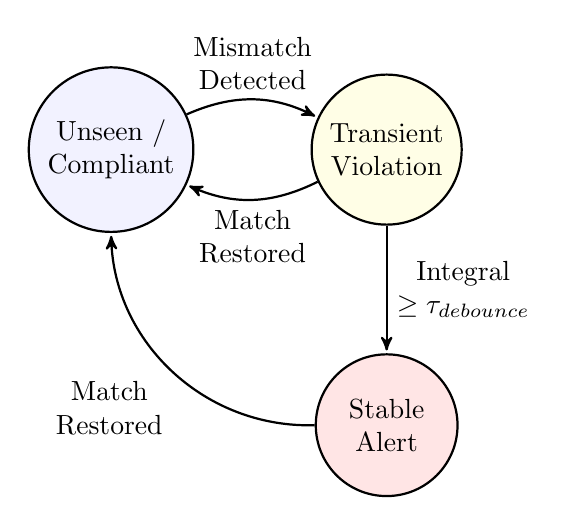
\begin{tikzpicture}[->, >=stealth', shorten >=1pt, auto, node distance=3.5cm, thick]
  \tikzstyle{state} = [circle, draw, minimum size=1.8cm, align=center, fill=blue!5]

  \node[state] (Unseen) {Unseen /\\Compliant};
  \node[state, fill=yellow!10] (Transient) [right of=Unseen] {Transient\\Violation};
  \node[state, fill=red!10] (Alert) [below of=Transient] {Stable\\Alert};

  \path 
    (Unseen) edge [bend left=25] node [above, align=center] {Mismatch\\Detected} (Transient)
    (Transient) edge [bend left=25] node [below, align=center] {Match\\Restored} (Unseen)
    (Transient) edge node [right, align=center] {Integral \\ $\ge \tau_{debounce}$} (Alert)
    (Alert) edge [bend left=45] node [below left, align=center] {Match \\ Restored} (Unseen);
\end{tikzpicture}
}
\caption{PCVF State Machine operating as a temporal low-pass filter. A student detected out-of-schedule enters the Transient state. An alert is only fired if the violation integral reaches the debounce threshold.}
\label{fig:fsm}
\end{figure}

% --- ALGORITHM 1: DATA SANITIZATION ---
\begin{algorithm}[htbp] % <--- CHANGED FROM [H] TO FIX SPACING
\caption{Temporal Debounce Filtering (PCVF)}
\begin{algorithmic}[1]
\REQUIRE Incoming Event Stream $S$, Threshold $\tau_{debounce}$
\ENSURE Validated Logic Events $E$
\FOR{each event $e$ in $S$}
    \STATE $ID \leftarrow e.identity$
    \STATE $Zone \leftarrow e.zone$
    \STATE $StateBuffer[ID].append(Zone, now())$
    \STATE
    \STATE \textbf{// Check contiguous duration in current zone}
    \IF{$\text{Duration}(StateBuffer[ID] == Zone) \ge \tau_{debounce}$}
        \STATE $E.add(ID, Zone)$ \COMMENT{Promote to stable event}
    \ELSE
        \STATE \textbf{Drop} \COMMENT{Filter as transient noise}
    \ENDIF
\ENDFOR
\RETURN $E$
\end{algorithmic}
\label{alg:sanitization}
\end{algorithm}

% ==========================================
% VI. BURST-ELASTIC READ OPTIMIZATION
% ==========================================
\section{Burst-Elastic Read Optimization}

Synchronized class transitions generate short bursts of extremely high event traffic across the campus network. Maintaining low latency under these conditions generally requires careful database engineering.

\subsection{Schema Partitioning Strategy}

The \texttt{student\_schedule} table is partitioned by \texttt{day\_of\_week}, immediately reducing search scope to a single partition. This reduces unnecessary cross-day scanning and constrains index traversal depth.

% --- LISTING 1: SQL SCHEMA ---
\begin{figure}[htbp] % <--- CHANGED FROM [H] TO FIX SPACING
\centering
\textbf{Listing 1: PostgreSQL Schedule Schema}
\begin{lstlisting}[language=SQL]
CREATE TABLE student_schedule (
  student_id VARCHAR(50) NOT NULL,
  day_of_week VARCHAR(3) CHECK (
    day_of_week IN ('MON','TUE','WED','THU','FRI')),
  start_time TIME NOT NULL,
  end_time TIME NOT NULL,
  expected_zone_id VARCHAR(50),
    
  PRIMARY KEY (student_id, day_of_week, start_time)
) PARTITION BY LIST (day_of_week);
\end{lstlisting}
\label{code:sql}
\end{figure}

When a stable event passes the PCVF layer, the logic issues a point-in-time query:
\begin{lstlisting}[language=SQL]
SELECT expected_zone_id FROM student_schedule 
WHERE student_id = ? AND day_of_week = ? 
AND start_time <= ? AND end_time >= ?
\end{lstlisting}

\subsection{Composite Temporal Indexing}
A composite B-Tree index \cite{b18} is applied across identity and temporal fields:
\begin{lstlisting}[language=SQL]
CREATE INDEX idx_temporal_lookup ON 
  student_schedule (student_id, day_of_week, start_time, end_time);
\end{lstlisting}
Given limited per-student schedule cardinality, this index rapidly narrows candidate intervals prior to temporal comparison \cite{b19}. The majority of latency arises from network and I/O overhead rather than index traversal.

\subsection{Connection Pooling and Capacity Stabilization}
During burst transitions, connection setup overhead can dominate query time. Without pooling:
\begin{equation}
T_{query} = T_{exec} + T_{conn}
\end{equation}
When $T_{conn}$ becomes significant, effective service capacity ($\mu$) collapses under high arrival rate ($\lambda$).

Transaction-level connection pooling removes this overhead from the critical path:
\begin{equation}
T_{query} \approx T_{exec}
\end{equation}
This data architecture adjustment significantly increases sustainable throughput and prevents connection exhaustion during thundering herd scenarios \cite{b20, b24}.

% ==========================================
% VII. EXPERIMENTAL EVALUATION
% ==========================================
\section{Experimental Evaluation}

\subsection{Evaluation Scope and Environment}
Evaluation focuses on two operational characteristics: lookup responsiveness and stability during burst traffic conditions. All results are derived from synthetic load testing designed to validate logical correctness and database throughput. The objective was not to model real campus demographics, but to stress the relational layer under controlled conditions.

Tests were executed on:
\begin{itemize}
    \item 16-core AMD EPYC server
    \item 64 GB RAM
    \item PostgreSQL 15
    \item \texttt{shared\_buffers} = 8GB
\end{itemize}
Each experiment was repeated five times with randomized identity distributions to smooth out skew from repeated key reuse patterns.

\subsection{Latency Decomposition}
Real-time responsiveness represents an important operational requirement. Rather than reporting a single aggregate metric, we decomposed latency into its constituent components.

\begin{table}[htbp]
\caption{Latency Decomposition per Event (Single Query)}
\begin{center}
\begin{tabular}{lcc}
\toprule
\textbf{Pipeline Stage} & \textbf{Time (ms)} & \textbf{Limiting Factor} \\
\midrule
Identity Resolution & - & Upstream Dependency \\
PCVF Debounce Check & $<0.1$ ms & CPU (In-Memory) \\
Schedule Lookup (DB) & 4.2 ms & Network / I/O \\
Predicate Logic Check & $<0.1$ ms & CPU \\
\textbf{Total Logic Delay} & \textbf{$\approx$ 4.4 ms} & \textbf{Interactive Range} \\
\bottomrule
\end{tabular}
\end{center}
\end{table}

The majority of latency originates from the relational lookup stage. Predicate evaluation itself contributes only a small portion of total latency relative to network and I/O costs. This reinforces an important design observation: compliance complexity does not meaningfully affect response time once the relational access path is optimized. Even under moderate concurrency, the evaluation layer consistently remained within single-digit millisecond latency.

\subsection{Throughput and Concurrency Stress Testing}
To evaluate burst resilience, the database was flooded with pre-generated identity tokens. Load was increased incrementally to 6,000 QPS.

Without connection pooling, the system began to degrade past 3,000 QPS. Tail latency rose sharply as connection overhead accumulated, confirming the expected $T_{conn}$ bottleneck.

With transaction-level pooling enabled, the latency curve flattened substantially. The database sustained approximately 5,000 QPS while maintaining sub-15 ms p99 latency ($\pm 1.2$ ms standard deviation). At $\sim$5,500 QPS, minor garbage collection pauses began contributing to the tail.

% --- FIGURE 2: THROUGHPUT ---
\begin{figure}[htbp]
\centering
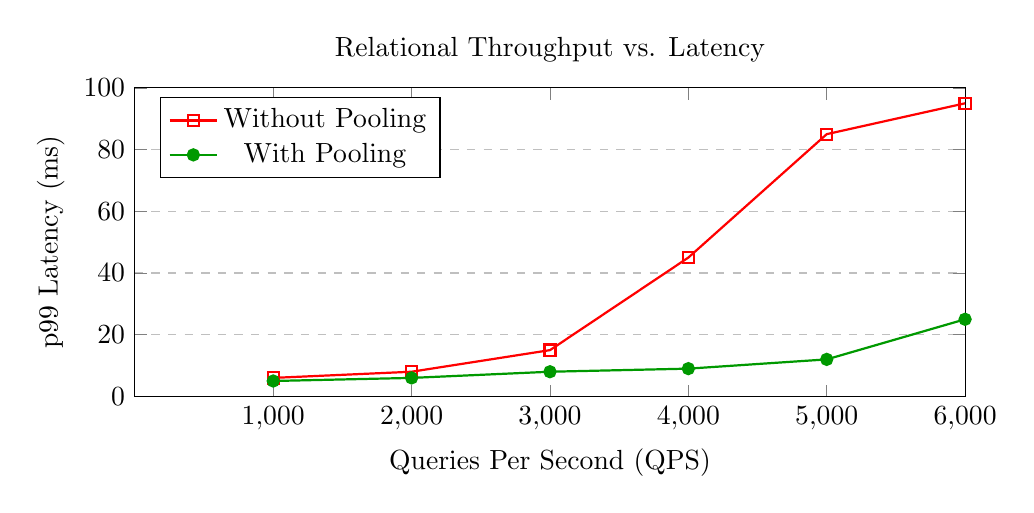
\begin{tikzpicture}
\begin{axis}[
    title={Relational Throughput vs. Latency},
    xlabel={Queries Per Second (QPS)},
    ylabel={p99 Latency (ms)},
    xmin=0, xmax=6000,
    ymin=0, ymax=100,
    xtick={1000, 2000, 3000, 4000, 5000, 6000},
    legend pos=north west,
    ymajorgrids=true,
    grid style=dashed,
    width=\columnwidth,
    height=5.5cm
]
\addplot[
    color=red,
    mark=square,
    thick
    ]
    coordinates {
    (1000, 6)(2000, 8)(3000, 15)(4000, 45)(5000, 85)(6000, 95)
    };
    \addlegendentry{Without Pooling}

\addplot[
    color=green!60!black,
    mark=*,
    thick
    ]
    coordinates {
    (1000, 5)(2000, 6)(3000, 8)(4000, 9)(5000, 12)(6000, 25)
    };
    \addlegendentry{With Pooling}
\end{axis}
\end{tikzpicture}
\caption{Throughput Stress Test. Without connection pooling (Red), connection exhaustion causes p99 latency to spike past 3,000 QPS. With pooling active (Green), the database sustains 5,000 QPS while maintaining sub-15ms p99 latency.}
\label{fig:throughput}
\end{figure}

The key takeaway is not peak throughput alone, but stability during synchronized transitions. Real campuses experience burst traffic when classes end simultaneously. Under these conditions, maintaining tail latency is more critical than maximizing theoretical throughput. The optimized relational configuration handled such bursts without observable cascading failure or connection exhaustion.

\subsection{Scenario-Based Operational Testing}
In addition to synthetic throughput tests, we evaluated specific behavioral scenarios to ensure logical correctness under edge conditions.

\begin{figure}[htbp]
\centering
\includegraphics[width=0.9\linewidth]{truancy_overlay.png}
\caption{Visual confirmation of the logic engine flagging a schedule conflict using synthetic agent data. The evaluation detects the mismatch between the physical zone (Canteen) and the scheduled requirement (Math Class).}
\label{fig:truancy}
\end{figure}

\begin{figure}[htbp]
\centering
\includegraphics[width=0.9\linewidth]{terminal_alert.png}
\caption{Real-time console output showing the flagging of the schedule violation event.}
\label{fig:terminal}
\end{figure}

\textbf{Scenario 1: Rapid Multi-Zone Transitions}\\
An agent traversed multiple restricted zones within a short time interval.
\textit{Result:} The PCVF state machine absorbed these transitions as transient noise. Because the violation integral never exceeded $\tau_{debounce}$, no alert was emitted. This confirmed that transit behavior does not trigger false escalation.

\textbf{Scenario 2: Intermittent Signal Loss}\\
An agent’s signal was intentionally dropped for two seconds before reappearing in the same zone.
\textit{Result:} The hysteresis buffer preserved the accumulated violation state. When the signal resumed, the debounce timer continued rather than resetting. Sustained violations were therefore still detected.

\textbf{Scenario 3: Backend Service Interruption}\\
The database connection was manually severed during active processing.
\textit{Result:} The logic trapped the exception and allowed the upstream event queue to buffer unread events. Upon restoration, the queue drained without data loss. No corrupted states were observed in the relational layer.

These controlled tests suggest that the evaluation logic remains stable under common operational disruptions.

% ==========================================
% VIII. DISCUSSION
% ==========================================
\section{Discussion}

\subsection{Logic Decoupling and Extensibility}
From a data evaluation perspective, isolating compliance checks within relational logic significantly improves extensibility across heterogeneous sensing technologies.

The compliance engine is agnostic to how identity is resolved. Optical recognition, RFID badges, WiFi triangulation, or future modalities can all feed the same tuple:
\begin{equation}
(ID, Zone, Timestamp)
\end{equation}
As long as this abstraction is respected, the relational predicate layer functions identically. This separation also simplifies logic evolution. Improvements to detection quality generally do not require modification of the evaluation query.

\subsection{Limits of Relational Evaluation}
The present system evaluates schedule compliance strictly through relational comparison. It does not attempt behavioral inference beyond zone adherence. While this constraint preserves clarity and auditability, it also limits scope.

For example:
\begin{itemize}
    \item Short-term collaborative movement between students is not analyzed.
    \item Behavioral intent is not inferred.
    \item Historical trajectory mining is not incorporated.
\end{itemize}

Future work could integrate temporal pattern analysis or trajectory clustering. However, such extensions would introduce additional complexity and potentially alter latency guarantees. The current design intentionally favors predictability over analytical breadth.

% ==========================================
% IX. CONCLUSION
% ==========================================
\section{Conclusion}
This study presented a data evaluation pipeline for continuously evaluating institutional schedule compliance using spatiotemporal predicate logic. By representing institutional rules as spatiotemporal predicates (CPEM) and applying a temporally smoothed violation filter (PCVF), the logic distinguishes sustained deviations from short-lived sensor noise.

From a performance perspective, sustained responsiveness depends less on predicate complexity and more on disciplined database engineering. Partitioned schema design, composite indexing, and transaction-level connection pooling enable the relational lookup to sustain burst traffic approaching 5,000 QPS while maintaining sub-15 ms tail latency.

The evaluation demonstrates that structured relational coordination can maintain stable lookup performance under distributed workloads. Relational responsiveness remains consistent across varying conditions.

% ==========================================
% REFERENCES
% ==========================================
\begin{thebibliography}{00}

\bibitem{b1} N. Min-Allah and S. Alrashed, "Smart campus: A sketch," \textit{Sustainable Cities and Society}, vol. 59, p. 102231, 2020.
\bibitem{b2} S. Dev and T. Patnaik, "Student Attendance System using Face Recognition," in \textit{ICOSEC}, IEEE, 2020, pp. 1-6.
\bibitem{b3} S. Bhattacharya, G. S. Nainala, P. Das, and A. Routray, "Smart attendance monitoring monitoring system (SAMS)," in \textit{ICALT}, IEEE, 2018, pp. 358-360.
\bibitem{b5} X. Wang, "Intelligent multi-camera video surveillance: A review," \textit{Pattern Recognition Letters}, vol. 34, no. 1, pp. 3-19, 2013.
\bibitem{b6} P. K. Atrey et al., "Multimodal fusion for multimedia analysis: A survey," \textit{Multimedia Systems}, vol. 16, no. 6, pp. 345-379, 2010.
\bibitem{b7} M. A. Khan et al., "Video Surveillance Anomaly Detection: A Review on Deep Learning Benchmarks," \textit{IEEE Access}, vol. 12, pp. 1-15, 2024.
\bibitem{b8} L. Zhang, "Spatio-Temporal Visual Analysis for Urban Traffic Characters Based on Video Surveillance Camera Data," \textit{ISPRS International Journal of Geo-Information}, vol. 10, no. 3, p. 177, 2021.
\bibitem{b9} A. Silberschatz, H. F. Korth, and S. Sudarshan, \textit{Database System Concepts}, 7th ed. McGraw-Hill, 2019.
\bibitem{b10} D. L. Hall and J. Llinas, "An introduction to multisensor data fusion," \textit{Proceedings of the IEEE}, vol. 85, no. 1, pp. 6-23, 1997.
\bibitem{b11} W. Shi et al., "Edge Computing: Vision and Challenges," \textit{IEEE Internet of Things Journal}, vol. 3, no. 5, pp. 637-646, 2016.
\bibitem{b12} M. Satyanarayarayanan, "The Emergence of Edge Computing," \textit{Computer}, vol. 50, no. 1, pp. 30-39, 2017.
\bibitem{b13} M. Stonebraker et al., "The 8 requirements of real-time stream processing," \textit{SIGMOD Record}, vol. 34, no. 4, pp. 42-47, 2005.
\bibitem{b14} T. Akidau et al., "The Dataflow Model: A Practical Approach to Balancing Correctness, Latency, and Cost in Massive-Scale, Unbounded, Out-of-Order Data Processing," \textit{Proc. VLDB Endow.}, vol. 8, no. 12, pp. 1792-1803, 2015.
\bibitem{b15} R. H. Güting et al., "A foundation for representing and querying moving objects," \textit{ACM Transactions on Database Systems (TODS)}, vol. 25, no. 1, pp. 1-42, 2000.
\bibitem{b16} Y. Zheng, "Trajectory data mining: an overview," \textit{ACM Transactions on Intelligent Systems and Technology (TIST)}, vol. 6, no. 3, pp. 1-41, 2015.
\bibitem{b17} E. Wu et al., "High-performance complex event processing over streams," \textit{SIGMOD}, pp. 407-418, 2006.
\bibitem{b18} D. Comer, "The ubiquitous B-tree," \textit{ACM Computing Surveys (CSUR)}, vol. 11, no. 2, pp. 121-137, 1979.
\bibitem{b19} B. Salzberg and V. J. Tsotras, "Comparison of access methods for time-evolving data," \textit{ACM Computing Surveys (CSUR)}, vol. 31, no. 2, pp. 158-221, 1999.
\bibitem{b20} S. Harizopoulos et al., "OLTP through the looking glass, and what we found there," \textit{SIGMOD}, pp. 981-992, 2008.
\bibitem{b21} J. M. Hellerstein et al., "Architecture of a Database System," \textit{Foundations and Trends in Databases}, vol. 1, no. 2, pp. 141-259, 2007.
\bibitem{b22} P. Carbone et al., "Apache Flink: Stream and Batch Processing in a Single Engine," \textit{IEEE Data Engineering Bulletin}, vol. 38, no. 4, pp. 28-38, 2015.
\bibitem{b23} Z. Zhou et al., "Edge Intelligence: Paving the Last Mile of Artificial Intelligence With Edge Computing," \textit{Proceedings of the IEEE}, vol. 107, no. 8, pp. 1738-1762, 2019.
\bibitem{b24} D. Abadi et al., "The Beckman Report on Database Research," \textit{SIGMOD Record}, vol. 43, no. 3, pp. 61-70, 2014.

\end{thebibliography}

\end{document}
